
\begin{figure}
  \centering
  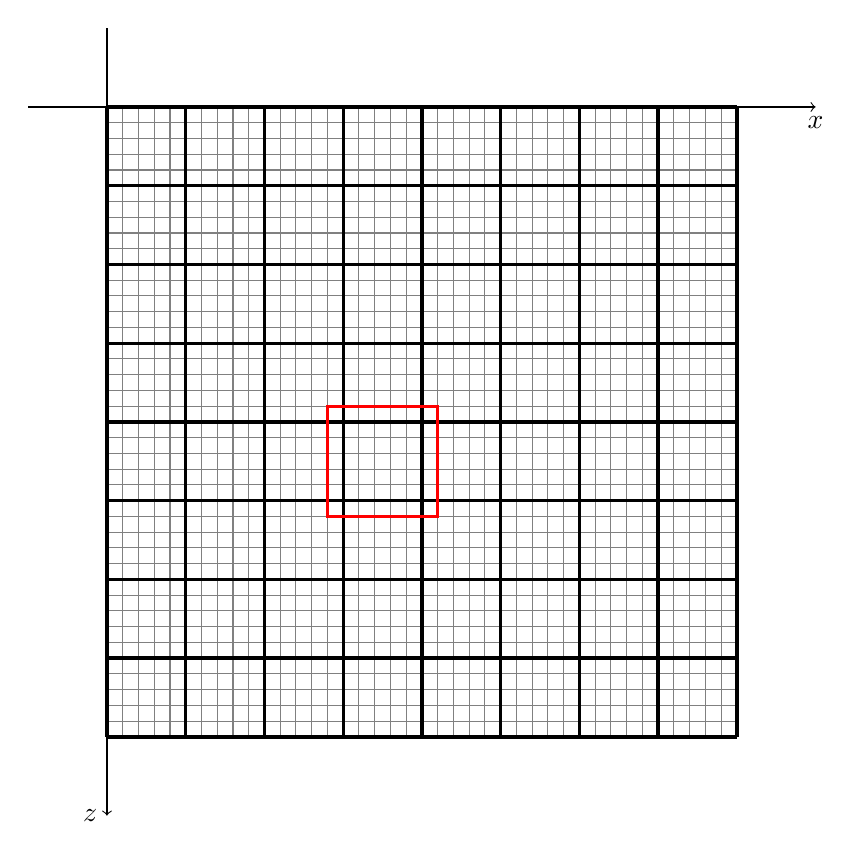
\begin{tikzpicture}
    % Draw x and y axis lines
    \draw [->] (-5,4) -- (5,4) node [below] {$x$};
    \draw [->] (-4,5) -- (-4,-5) node [left] {$z$};
    \draw[step=0.2cm,color=gray] (-4,-4) grid (4,4);   
    \draw[very thick] (-4,-4)--(-4,4);
    \draw[very thick] (4,-4)--(4,4);
    \draw[very thick] (3,-4)--(3,4);
    \draw[very thick] (2,-4)--(2,4);
    \draw[very thick] (1,-4)--(1,4);
    \draw[very thick] (0,-4)--(0,4);
    \draw[very thick] (-3,-4)--(-3,4);
    \draw[very thick] (-2,-4)--(-2,4);
    \draw[very thick] (-1,-4)--(-1,4);
    \draw[very thick] (-4,-4)--(4,-4);
    \draw[very thick] (-4,-3)--(4,-3);
    \draw[very thick] (-4,-2)--(4,-2);
    \draw[very thick] (-4,-1)--(4,-1);
    \draw[very thick] (-4,0)--(4,0);
    \draw[very thick] (-4,4)--(4,4);
    \draw[very thick] (-4,3)--(4,3);
    \draw[very thick] (-4,2)--(4,2);
    \draw[very thick] (-4,1)--(4,1);    
    \draw [very thick,red] (-1.2,-1.2) rectangle (0.2,0.2);    
  \end{tikzpicture}
\end{figure}
